% =============================================================================
%  Exosuit Cable Stiffness Control and Co-Contraction Mechanism
%  Addresses: coupling between joint rotation and stiffness modulation
% =============================================================================

\documentclass[11pt, a4paper]{article}

\usepackage{amsmath, amssymb, bm}
\usepackage{geometry}
\usepackage{hyperref}
\usepackage{booktabs}
\usepackage{xcolor}
\usepackage{graphicx}
\usepackage{tikz}
\usetikzlibrary{arrows.meta, decorations.pathmorphing, positioning, calc, patterns}
\usepackage{cleveref}
\usepackage[backgroundcolor=blue!5, linecolor=blue!40, linewidth=1pt,
            innertopmargin=6pt, innerbottommargin=6pt,
            innerleftmargin=7pt, innerrightmargin=7pt]{mdframed}

\geometry{margin=2.2cm}

% ── Standard project macros ──────────────────────────────────────────────────
\newcommand{\bq}{\bm{q}}
\newcommand{\bp}{\bm{p}}
\newcommand{\bu}{\bm{u}}
\newcommand{\btau}{\bm{\tau}}
\newcommand{\bF}{\bm{F}}
\newcommand{\bJ}{\bm{J}}
\newcommand{\bM}{\bm{M}}
\newcommand{\bC}{\bm{C}}
\newcommand{\bG}{\bm{G}}

\title{\textbf{Exosuit Cable Stiffness Control \\and Co-Contraction Mechanism}\\
       \large \texttt{cable/cable\_with\_exo\_springs.py}}
\date{April 2026}
\author{Isaac-sim robotics notes}

\begin{document}
\maketitle

% ─────────────────────────────────────────────────────────────────────────────
\section{Overview}
% ─────────────────────────────────────────────────────────────────────────────

The cup manipulator uses \textbf{two independent cable systems} acting on the
elbow joint~$q_2$:

\begin{enumerate}
    \item \textbf{Drive cables} (green/red, bottom) --- antagonistic belt-drive
          via a Series Elastic Actuator (SEA).  These cables \emph{actuate}
          the joint: one cable pulls for positive torque, the other for
          negative torque.
    \item \textbf{Exosuit cables} (orange/magenta, top) --- routed over
          link-1 and elbow pulleys with a compliant spring element between
          the elbow pulley exit and the link-2 anchor.  These cables
          \emph{do not drive the joint} during normal operation.  They
          provide on-demand stiffness when activated by the upper motors.
\end{enumerate}

\begin{mdframed}
\textbf{Key design question (Thrish, April 2026):}
\emph{``Are the two purple motors driving only stiffness / co-contraction,
or are they driving the joint too?''}

\medskip\noindent
\textbf{Answer:} The top motors drive \emph{only stiffness}.  The bottom
cables drive the joint.  Stiffness control kicks in only when needed
(disturbance rejection), not during free joint rotation.
\end{mdframed}

% ─────────────────────────────────────────────────────────────────────────────
\section{Physical Architecture}
% ─────────────────────────────────────────────────────────────────────────────

\begin{figure}[h]
\centering
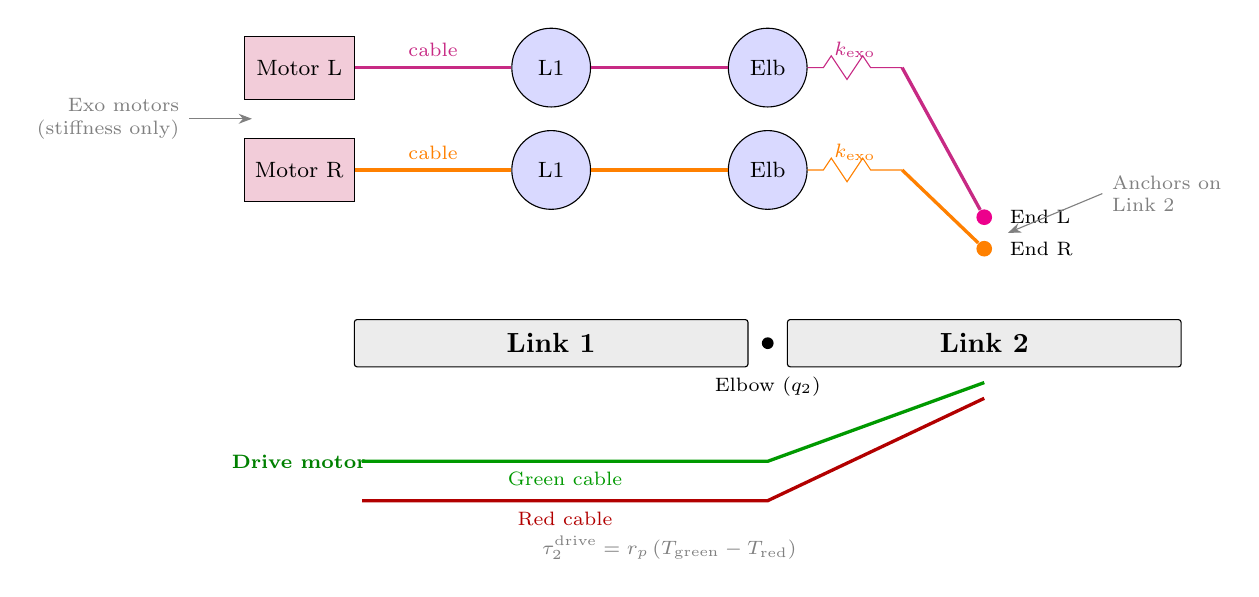
\begin{tikzpicture}[
    >=Stealth,
    pulley/.style={circle, draw, fill=blue!15, minimum size=10mm, font=\footnotesize},
    motor/.style={rectangle, draw, fill=purple!20, minimum width=14mm,
                  minimum height=8mm, font=\footnotesize},
    spring/.style={decorate, decoration={zigzag, segment length=4mm,
                   amplitude=1.5mm, pre length=2mm, post length=2mm}},
    cable/.style={very thick},
    link/.style={draw, fill=gray!15, minimum height=6mm, rounded corners=1pt},
]
    % ── Links ─────────────────────────────────────
    \node[link, minimum width=50mm] (link1) at (0,0) {\textbf{Link 1}};
    \node[link, minimum width=50mm] (link2) at (5.5,0) {\textbf{Link 2}};
    \node[fill=black, circle, inner sep=1.5pt] at (2.75,0) {};
    \node[below, font=\scriptsize] at (2.75,-0.3) {Elbow ($q_2$)};

    % ── Drive cable system (bottom) ──────────────
    \node[font=\scriptsize\bfseries, color=green!50!black] at (-3.2,-1.5) {Drive motor};
    \draw[cable, green!60!black] (-2.4,-1.5) -- node[below, font=\scriptsize, pos=0.5]
         {Green cable} (2.75,-1.5) -- (5.5,-0.5);
    \draw[cable, red!70!black]   (-2.4,-2.0) -- node[below, font=\scriptsize, pos=0.5]
         {Red cable}   (2.75,-2.0) -- (5.5,-0.7);
    \node[font=\scriptsize, color=gray] at (1.5,-2.6) {%
      $\tau_2^{\text{drive}} = r_p\,(T_{\text{green}} - T_{\text{red}})$};

    % ── Exo cable system (top) ────────────────────
    % Right exo cable (orange)
    \node[motor] (motorR) at (-3.2, 2.2) {Motor R};
    \node[pulley] (link1pR) at (0, 2.2) {L1};
    \node[pulley] (elbowpR) at (2.75, 2.2) {Elb};
    \node[circle, fill=orange, inner sep=2pt] (endR) at (5.5, 1.2) {};
    \node[right, font=\scriptsize] at (5.7, 1.2) {End R};

    \draw[cable, orange]  (motorR.east) -- node[above, font=\scriptsize] {cable}
                          (link1pR.west);
    \draw[cable, orange]  (link1pR.east) -- (elbowpR.west);
    \draw[spring, orange] (elbowpR.east) -- node[above, font=\scriptsize]
         {$k_{\text{exo}}$} ++(1.2,0) coordinate (spR);
    \draw[cable, orange]  (spR) -- (endR);

    % Left exo cable (magenta)
    \node[motor] (motorL) at (-3.2, 3.5) {Motor L};
    \node[pulley] (link1pL) at (0, 3.5) {L1};
    \node[pulley] (elbowpL) at (2.75, 3.5) {Elb};
    \node[circle, fill=magenta, inner sep=2pt] (endL) at (5.5, 1.6) {};
    \node[right, font=\scriptsize] at (5.7, 1.6) {End L};

    \draw[cable, magenta!80!black] (motorL.east) -- node[above, font=\scriptsize]
         {cable} (link1pL.west);
    \draw[cable, magenta!80!black] (link1pL.east) -- (elbowpL.west);
    \draw[spring, magenta!80!black] (elbowpL.east) -- node[above, font=\scriptsize]
         {$k_{\text{exo}}$} ++(1.2,0) coordinate (spL);
    \draw[cable, magenta!80!black] (spL) -- (endL);

    % ── Annotations ───────────────────────────────
    \draw[<-, gray, thin] (5.8, 1.4) -- ++(1.2, 0.5)
         node[right, font=\scriptsize, align=left] {Anchors on\\Link 2};
    \draw[<-, gray, thin] (-3.8, 2.85) -- ++(-0.8, 0)
         node[left, font=\scriptsize, align=right] {Exo motors\\(stiffness only)};
\end{tikzpicture}
\caption{Dual cable architecture.  Drive cables (bottom, green/red) actuate
the elbow joint.  Exo cables (top, orange/magenta) route through link-1 and
elbow pulleys with a spring element before the link-2 anchor.}
\label{fig:architecture}
\end{figure}

\subsection{Cable routing summary}

\begin{table}[h]
\centering
\begin{tabular}{@{}llll@{}}
\toprule
\textbf{Cable}  & \textbf{Route} & \textbf{Role} & \textbf{Actuator} \\
\midrule
Green (drive)  & DrivePulley $\to$ Idler R $\to$ BigPulley $\to$ End L
               & Joint torque $+\tau_2$ & SEA motor \\
Red (drive)    & DrivePulley $\to$ Idler L $\to$ BigPulley $\to$ End R
               & Joint torque $-\tau_2$ & SEA motor \\
\midrule
Orange (exo R) & Start R $\to$ Link1 Pulley R $\to$ Elbow Pulley R
               $\xrightarrow{\text{spring}}$ End R
               & Stiffness $+$ & Exo motor R \\
Magenta (exo L)& Start L $\to$ Link1 Pulley L $\to$ Elbow Pulley L
               $\xrightarrow{\text{spring}}$ End L
               & Stiffness $+$ & Exo motor L \\
\bottomrule
\end{tabular}
\caption{Four cable routes on the cup manipulator.}
\label{tab:cables}
\end{table}

% ─────────────────────────────────────────────────────────────────────────────
\section{Operating Modes}
% ─────────────────────────────────────────────────────────────────────────────

\subsection{Mode 1: Free rotation (no disturbance)}

During normal operation the exo motors are \textbf{inactive} (zero command).
The exo cable springs sit in their natural rest length~$l_0$:
%
\begin{align}
    \delta_{\text{exo}} &= 0, &
    F_{\text{exo}} &= 0, &
    \tau_2^{\text{exo}} &= 0.
\end{align}
%
Joint motion is governed entirely by the drive cables:
%
\begin{equation}
    \bM(\bq)\,\ddot{\bq} + \bC(\bq,\dot{\bq})\,\dot{\bq} + \bG(\bq)
    = \begin{bmatrix} 0 \\ \tau_2^{\text{drive}} \end{bmatrix}.
\end{equation}
%
The exo springs are slack $\Rightarrow$ \textbf{zero coupling} between stiffness
and rotation.  Joint stiffness equals the intrinsic drive-cable SEA stiffness
$k_{\text{SEA}}$ alone.

\subsection{Mode 2: Disturbance rejection (co-contraction)}

When link~2 contacts an object, the sudden deceleration
$|\ddot{q}_2| > \ddot{q}_{\text{thresh}}$ triggers the exo motors.
Both exo motors pull their cables simultaneously
(``co-contraction''), stretching both springs:
%
\begin{align}
    \delta_R &= l_{m,R} - r_{\text{elb}}\,q_2, &
    \delta_L &= l_{m,L} + r_{\text{elb}}\,q_2, \\[4pt]
    F_R &= k_{\text{exo}}\,\delta_R + b_{\text{exo}}\,\dot{\delta}_R, \qquad &
    F_L &= k_{\text{exo}}\,\delta_L + b_{\text{exo}}\,\dot{\delta}_L.
\end{align}
%
The net exo torque on the elbow is:
%
\begin{equation}\label{eq:tau_exo}
    \tau_2^{\text{exo}}
    = r_{\text{elb}}\bigl(-F_R + F_L\bigr).
\end{equation}
%
Because both cables are pulled equally, the torque contributions
\emph{partially cancel}, leaving a small restoring torque that drives $q_2$
back toward the nominal position.  The dominant effect is an increase in
\textbf{apparent joint stiffness}:
%
\begin{equation}\label{eq:stiffness}
    \boxed{%
    k_{\text{eff}}
    = k_{\text{SEA}} + 2\,k_{\text{exo}}\,r_{\text{elb}}^2
    }
\end{equation}
%
where the factor of~2 arises from both (R and L) springs acting
simultaneously.

\begin{mdframed}
\textbf{Co-contraction principle:}
When both exo motors pull equally, the net \emph{torque} on the joint is
approximately zero (symmetric cancellation), but the \emph{stiffness} doubles
because each spring resists any deviation from the current position.  This is
analogous to biological antagonistic co-contraction where simultaneous
activation of agonist and antagonist muscles increases joint impedance without
changing the equilibrium position.
\end{mdframed}

% ─────────────────────────────────────────────────────────────────────────────
\section{Worked Example: Disturbance at $q_2 = 30°$}
\label{sec:example}
% ─────────────────────────────────────────────────────────────────────────────

\begin{mdframed}
\textbf{What is the nominal position?}
The \emph{nominal position} $q_2^{\text{nom}}$ is the joint angle at the
instant the disturbance is detected --- i.e.\ the angle the exo system
``captures'' and tries to restore.  It is \textbf{not} a fixed home angle;
it is whatever angle the joint was at when the impact happened.
\end{mdframed}

\noindent
Consider a concrete scenario with representative numbers:

\begin{table}[h]
\centering
\begin{tabular}{@{}ll@{}}
\toprule
\textbf{Parameter} & \textbf{Value} \\
\midrule
Exo spring stiffness $k_{\text{exo}}$      & $200\;\text{N/m}$ \\
Elbow pulley radius  $r_{\text{elb}}$      & $0.032\;\text{m}$ \\
Pretension pull      $\Delta l$            & $0.005\;\text{m}$ (5\,mm) \\
Activation threshold $\ddot{q}_{\text{thresh}}$ & $50\;\text{rad/s}^2$ \\
\bottomrule
\end{tabular}
\end{table}

\subsection*{Timeline}

\begin{enumerate}
    \item[\textbf{T$_0$}:]
        Joint rotating freely at $q_2 = 30°\;(0.524\;\text{rad})$.
        Exo motors OFF.  Springs at rest.
        \[
            F_R = F_L = 0, \qquad \tau_2^{\text{exo}} = 0.
        \]

    \item[\textbf{T$_1$}:]
        Link~2 strikes an object.  Impact deflects the joint to
        $q_2 = 45°\;(0.785\;\text{rad})$ --- a disturbance of $+15°$.
        The acceleration spike reaches $|\ddot{q}_2| = 120\;\text{rad/s}^2
        > 50$ (threshold).

    \item[\textbf{T$_2$}:]
        Disturbance detector fires.  Exo controller captures the
        \textbf{pre-disturbance angle} as the nominal position:
        \[
            \boxed{q_2^{\text{nom}} = 30°}
        \]
        Both exo motors pull with symmetric commands:
        \begin{align}
            l_{m,R}^{\text{cmd}} &= r_{\text{elb}}\,q_2^{\text{nom}} + \Delta l
                = 0.032 \times 0.524 + 0.005
                = 0.0218\;\text{m}, \\
            l_{m,L}^{\text{cmd}} &= -r_{\text{elb}}\,q_2^{\text{nom}} + \Delta l
                = -0.032 \times 0.524 + 0.005
                = -0.0118\;\text{m}.
        \end{align}

    \item[\textbf{T$_3$}:]
        Joint is at $q_2 = 45°$ (deflected).  Spring extensions:
        \begin{align}
            \delta_R &= l_{m,R} - r_{\text{elb}}\,q_2
                     = 0.0218 - 0.032 \times 0.785 = -0.0033\;\text{m}, \\
            \delta_L &= l_{m,L} + r_{\text{elb}}\,q_2
                     = -0.0118 + 0.032 \times 0.785 = 0.0133\;\text{m}.
        \end{align}
        Spring forces (ignoring damping for clarity):
        \begin{align}
            F_R &= k_{\text{exo}} \cdot \max(\delta_R,\, 0) = 200 \times 0 = 0\;\text{N}
                   \quad \text{(cable slack)}, \\
            F_L &= k_{\text{exo}} \cdot \delta_L = 200 \times 0.0133 = 2.67\;\text{N}.
        \end{align}
        Net exo restoring torque:
        \[
            \tau_2^{\text{exo}} = r_{\text{elb}}\,(-F_R + F_L)
            = 0.032 \times (0 + 2.67)
            = +0.085\;\text{N\,m}.
        \]
        This torque acts \textbf{in the negative direction} relative to the
        deflection (pulling $q_2$ from $45°$ back toward $30°$).

    \item[\textbf{T$_4$}:]
        The restoring torque (combined with drive-cable controller) brings
        $q_2$ back toward $30°$.  At $q_2 = q_2^{\text{nom}} = 30°$ the
        spring forces become symmetric and the net exo torque is zero ---
        the joint settles at the captured nominal position.

    \item[\textbf{T$_5$}:]
        Acceleration drops below threshold.  Exo motors release.  Springs
        return to rest.  Joint continues under drive-cable control alone.
\end{enumerate}

\subsection*{Stiffness increase during co-contraction}

While both exo cables are active, any small deviation $\Delta q_2$ from
$q_2^{\text{nom}}$ is resisted by an additional restoring torque:
\[
    \Delta\tau \approx 2\,k_{\text{exo}}\,r_{\text{elb}}^2\,\Delta q_2
    = 2 \times 200 \times 0.032^2 \times \Delta q_2
    = 0.41\;\text{N\,m/rad} \times \Delta q_2.
\]
So the effective stiffness increase is $\Delta k = 0.41\;\text{N\,m/rad}$,
added on top of the drive-cable SEA stiffness.

\begin{mdframed}
\textbf{Key insight:} The nominal position is \emph{not} hard-coded.
It is the joint angle at the moment of impact detection.  If the joint is
at $10°$ when hit, the exo system restores to $10°$.  If at $60°$, it
restores to $60°$.  The exo cables act like a temporary ``clamp'' around
wherever the joint happened to be.
\end{mdframed}

% ─────────────────────────────────────────────────────────────────────────────
\section{Achieving Co-Contraction Without Affecting Rotation}
\label{sec:coupling}
% ─────────────────────────────────────────────────────────────────────────────

Thrish raised a key requirement:

\begin{quote}
\emph{``There should be a coupling.  The joint stiffness should remain the
same when it rotates, and stiffness control should kick in only when it is
needed.''}
\end{quote}

\noindent
This is achieved through three design features:

\subsection{Spring decoupling}

The spring element between the elbow pulley and the link-2 anchor is the
critical decoupling component.  When the exo motors are off:

\begin{itemize}
    \item The springs are at rest length ($\delta_{\text{exo}} = 0$).
    \item Joint rotation changes the cable geometry but does \emph{not}
          stretch the springs (no pretension).
    \item Therefore $F_{\text{exo}} = 0$ regardless of $q_2$.
\end{itemize}

\noindent
Only when the exo motors actively pull (creating pretension) does the spring
force depend on $q_2$.

\subsection{Symmetric activation for pure stiffness}

When both exo motors are commanded with the \emph{same} displacement
$l_m^{\text{cmd}}$, the net torque is:
%
\begin{equation}
    \tau_2^{\text{exo}}
    = r_{\text{elb}}\bigl(
        -k_{\text{exo}}(l_m - r_{\text{elb}}\,q_2)
        +k_{\text{exo}}(l_m + r_{\text{elb}}\,q_2)
      \bigr)
    = 2\,k_{\text{exo}}\,r_{\text{elb}}^2\,q_2.
\end{equation}
%
This is a \textbf{pure spring-like restoring torque} centred at $q_2 = 0$.
The stiffness increase is $\Delta k = 2\,k_{\text{exo}}\,r_{\text{elb}}^2$,
independent of the drive cable command.

To centre the stiffness around an \emph{arbitrary} nominal angle
$q_2^{\text{nom}}$, the motors command:
%
\begin{equation}
    l_{m,R}^{\text{cmd}} = r_{\text{elb}}\,q_2^{\text{nom}} + \Delta l, \qquad
    l_{m,L}^{\text{cmd}} = -r_{\text{elb}}\,q_2^{\text{nom}} + \Delta l,
\end{equation}
%
where $\Delta l > 0$ is the pretension distance.  This shifts the zero-torque
point to $q_2^{\text{nom}}$ while maintaining symmetric stiffness.

\subsection{Threshold-based activation}

The exo controller activates only when a disturbance is detected:
%
\begin{equation}
    \bu_{\text{exo}} =
    \begin{cases}
        \Delta l \cdot \bm{1} & \text{if } |\ddot{q}_2| > \ddot{q}_{\text{thresh}}, \\
        0                     & \text{otherwise}.
    \end{cases}
\end{equation}
%
This ensures:
\begin{itemize}
    \item \textbf{Free rotation:} Joint moves with drive-cable stiffness only
          ($k_{\text{SEA}}$).  No parasitic torque from exo cables.
    \item \textbf{Impact:} Acceleration spike triggers co-contraction.
          Effective stiffness jumps to $k_{\text{SEA}} + 2k_{\text{exo}}
          r_{\text{elb}}^2$.
    \item \textbf{Recovery:} Springs pull link~2 back toward the nominal
          position.  Once $|\ddot{q}_2|$ drops below threshold, exo motors
          release and springs return to rest.
\end{itemize}

% ─────────────────────────────────────────────────────────────────────────────
\section{Dynamics Summary}
% ─────────────────────────────────────────────────────────────────────────────

The full elbow dynamics with both cable systems:
%
\begin{equation}\label{eq:full}
    M_{22}\,\ddot{q}_2 + c_2(\bq,\dot{\bq}) + g_2(\bq)
    = \underbrace{r_p\,(T_{\text{green}} - T_{\text{red}})}_{\text{drive cable}}
    \;+\;
    \underbrace{r_{\text{elb}}\,(-F_R + F_L)}_{\text{exo cables (when active)}}.
\end{equation}

\begin{table}[h]
\centering
\begin{tabular}{@{}lll@{}}
\toprule
\textbf{Symbol} & \textbf{Description} & \textbf{Units} \\
\midrule
$k_{\text{SEA}}$        & Drive cable spring stiffness       & N/m \\
$k_{\text{exo}}$        & Exo cable spring stiffness         & N/m \\
$b_{\text{exo}}$        & Exo cable spring damping           & N\,s/m \\
$r_p$                   & Drive big-pulley radius            & m \\
$r_{\text{elb}}$        & Exo elbow-pulley radius ($0.032$)  & m \\
$\Delta l$              & Co-contraction pretension distance  & m \\
$\ddot{q}_{\text{thresh}}$ & Activation threshold            & rad/s$^2$ \\
$q_2^{\text{nom}}$      & Nominal elbow angle (stiffness centre) & rad \\
\bottomrule
\end{tabular}
\caption{Exosuit stiffness control parameters.}
\label{tab:params}
\end{table}

% ─────────────────────────────────────────────────────────────────────────────
\section{Block Diagram: Control Flow}
% ─────────────────────────────────────────────────────────────────────────────

\begin{figure}[h]
\centering
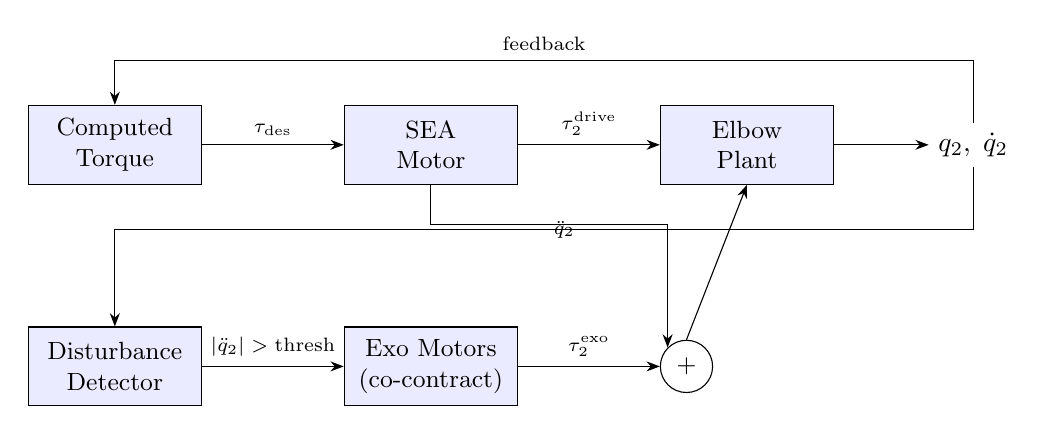
\begin{tikzpicture}[
    >=Stealth,
    block/.style={rectangle, draw, fill=blue!8, minimum width=22mm,
                  minimum height=10mm, font=\small, align=center},
    sum/.style={circle, draw, minimum size=6mm, font=\small},
    node distance=14mm and 18mm,
]
    % Drive path
    \node[block] (ct) {Computed\\Torque};
    \node[block, right=of ct] (sea) {SEA\\Motor};
    \node[block, right=of sea] (plant) {Elbow\\Plant};
    \node[right=12mm of plant] (q2) {$q_2,\;\dot{q}_2$};

    \draw[->] (ct) -- node[above, font=\scriptsize] {$\tau_{\text{des}}$} (sea);
    \draw[->] (sea) -- node[above, font=\scriptsize] {$\tau_2^{\text{drive}}$} (plant);
    \draw[->] (plant) -- (q2);

    % Exo path
    \node[block, below=18mm of ct] (detect) {Disturbance\\Detector};
    \node[block, right=of detect] (exo) {Exo Motors\\(co-contract)};
    \node[sum, right=of exo] (sum) {$+$};

    \draw[->] (q2.south) -- ++(0,-0.8) -| (detect.north)
         node[near start, right, font=\scriptsize] {$\ddot{q}_2$};
    \draw[->] (detect) -- node[above, font=\scriptsize]
         {$|\ddot{q}_2|>\text{thresh}$} (exo);
    \draw[->] (exo) -- node[above, font=\scriptsize]
         {$\tau_2^{\text{exo}}$} (sum);
    \draw[->] (sum.north) -- (plant.south);
    \draw[->] (sea.south) -- ++(0,-0.5) -| (sum.north west);

    % Feedback
    \draw[->] (q2.north) -- ++(0,0.8) -| (ct.north)
         node[near start, above, font=\scriptsize] {feedback};
\end{tikzpicture}
\caption{Control block diagram.  The drive path (top) runs continuously.
The exo path (bottom) activates only on disturbance detection.}
\label{fig:control}
\end{figure}

% ─────────────────────────────────────────────────────────────────────────────
\section{Comparison with Biological Co-Contraction}
% ─────────────────────────────────────────────────────────────────────────────

\begin{table}[h]
\centering
\begin{tabular}{@{}lll@{}}
\toprule
\textbf{Aspect} & \textbf{Biological} & \textbf{Our mechanism} \\
\midrule
Agonist/Antagonist  & Biceps/Triceps         & Drive green/red cables \\
Co-contraction      & Both muscles activate  & Both exo motors pull \\
Stiffness source    & Muscle short-range stiffness & Exo spring $k_{\text{exo}}$ \\
Activation trigger  & Reflex (stretch reflex) & $|\ddot{q}_2| > $ threshold \\
Decoupling          & Reciprocal inhibition   & Spring at rest $\Rightarrow F=0$ \\
\bottomrule
\end{tabular}
\caption{Biological co-contraction analogy.}
\label{tab:bio}
\end{table}

\begin{mdframed}
\textbf{Summary of the coupling answer:}
The exo springs provide a natural \emph{mechanical decoupling}.  When the
exo motors are off, the springs are slack and exert zero force regardless of
joint angle, so stiffness ``remains the same when it rotates.''  When the
exo motors pull (both simultaneously), stiffness increases symmetrically
around the nominal position.  The drive cables remain the sole actuator for
joint trajectory tracking.  This is the ``coupling'' Thrish described:
stiffness control that is independent of and additive to joint rotation
control.
\end{mdframed}

% ─────────────────────────────────────────────────────────────────────────────
\section{Alternative Routing: Encoder-Tracking Steppers}
\label{sec:chris}
% ─────────────────────────────────────────────────────────────────────────────

Chris Kalogroulis (April 2026) proposed a simplified exosuit architecture.
Both methods share the same \textbf{motor pulleys} at the base and route
cables along link~1 to the elbow.  The single difference is at the elbow:
instead of two small offset pulleys ($r_{\text{elb}} = 32\;\text{mm}$,
located $103\;\text{mm}$ before the joint axis), Chris replaces them with
\textbf{one pulley centred directly on the elbow joint axis}, matching the
driven big-pulley geometry (see image below).

\begin{enumerate}
    \item \textbf{Same cable route as drive cables} --- exo cables follow
          the same path: motor pulley $\to$ along link~1 $\to$
          wrap around a pulley at the elbow $\to$ spring $\to$ anchor on
          link~2.  The routing is identical to the green/red drive cables;
          the only change is that the elbow pulley sits \emph{on the joint
          axis} instead of being offset.
    \item \textbf{1:1 pulley ratio} --- the new exo elbow pulley has the
          same diameter as the driven big-pulley
          ($r_{\text{cp}} = r_p = 47.75\;\text{mm}$), so one motor
          revolution equals one joint revolution.
    \item \textbf{Encoder-tracking steppers} --- each exo stepper motor
          continuously tracks the joint encoder in real time, feeding cable
          at the rate the joint moves.  This keeps both cables taut at all
          times without active co-contraction logic.
    \item \textbf{Force via angular offset} --- to apply stiffness, the
          controller adds a small angular offset $\Delta\theta$ to both
          stepper commands simultaneously:
          %
          \begin{equation}\label{eq:chris-force}
              F_{\text{exo}} = k_{\text{exo}} \cdot r_{\text{cp}} \cdot \Delta\theta.
          \end{equation}
          %
          Because both cables are offset equally, the result is symmetric
          pretension (increased stiffness) with no net torque at the nominal
          position.
    \item \textbf{Latency is the key test} --- the feasibility of this
          approach depends on the stepper--encoder loop bandwidth.  If the
          stepper cannot track fast joint motions, the cable will alternately
          go slack and snap taut.
\end{enumerate}

\begin{mdframed}
\textbf{Prototype strategy (Chris):}
Build a quick first exosuit with \emph{only} the stepper motors and encoder
--- no springs, no CubeMars drive motors.  Measure the tracking latency.  If
steppers can follow the joint encoder with $<5\;\text{ms}$ lag, the full
system is viable.
\end{mdframed}

% ── Side-by-side routing comparison ──────────────────────────────────────────
\begin{figure}[h]
\centering
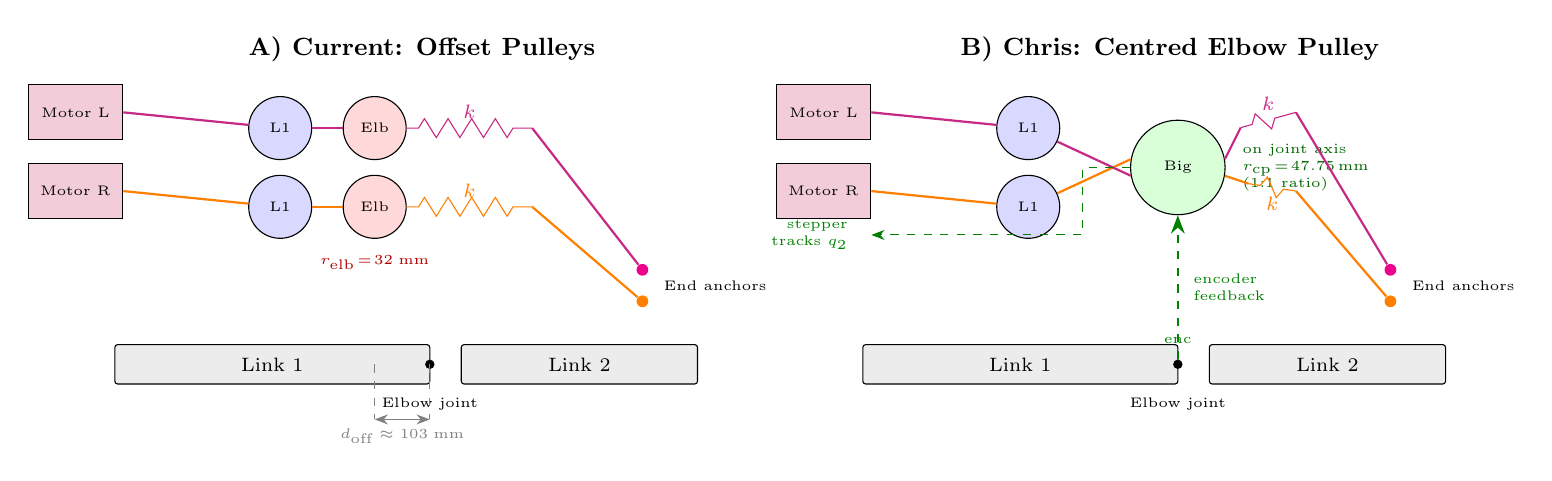
\begin{tikzpicture}[
    >=Stealth,
    pulley/.style={circle, draw, fill=blue!15, minimum size=8mm,
                   font=\scriptsize},
    motor/.style={rectangle, draw, fill=purple!20, minimum width=12mm,
                  minimum height=7mm, font=\scriptsize},
    spring/.style={decorate, decoration={zigzag, segment length=3mm,
                   amplitude=1.2mm, pre length=1.5mm, post length=1.5mm}},
    cable/.style={thick},
    link/.style={draw, fill=gray!15, minimum height=5mm, rounded corners=1pt,
                 font=\scriptsize},
    joint/.style={fill=black, circle, inner sep=1.2pt},
    lbl/.style={font=\scriptsize},
]

% ═══════════════════════════════════════════════════════════════════════════
%  LEFT: Current design (offset pulleys)
% ═══════════════════════════════════════════════════════════════════════════
\begin{scope}[shift={(0,0)}]
    \node[font=\small\bfseries] at (2.2,4.0) {A) Current: Offset Pulleys};

    % Links
    \node[link, minimum width=40mm] (L1a) at (0.3,0) {Link 1};
    \node[link, minimum width=30mm] (L2a) at (4.2,0) {Link 2};
    \node[joint] (Ja) at (2.3,0) {};
    \node[below, font=\tiny] at (2.3,-0.3) {Elbow joint};

    % Motor pulleys at base (both methods have these)
    \node[motor] (MRa) at (-2.2,2.2) {\tiny Motor R};
    \node[motor] (MLa) at (-2.2,3.2) {\tiny Motor L};

    % Link1 pulleys (offset, on link1 body)
    \node[pulley] (P1Ra) at (0.4,2.0) {\tiny L1};
    \node[pulley] (P1La) at (0.4,3.0) {\tiny L1};

    % TWO offset elbow pulleys (r=32mm, 103mm before joint axis)
    \node[pulley, fill=red!15] (PERa) at (1.6,2.0) {\tiny Elb};
    \node[pulley, fill=red!15] (PELa) at (1.6,3.0) {\tiny Elb};

    % End anchors on link2
    \node[circle, fill=orange, inner sep=1.5pt] (ERa) at (5.0,0.8) {};
    \node[circle, fill=magenta, inner sep=1.5pt] (ELa) at (5.0,1.2) {};
    \node[right, font=\tiny] at (5.15,1.0) {End anchors};

    % Right cable: Motor → L1 → offset Elbow → spring → end
    \draw[cable, orange] (MRa.east) -- (P1Ra);
    \draw[cable, orange] (P1Ra) -- (PERa);
    \coordinate (spRa_end) at (3.6,2.0);
    \draw[spring, orange] (PERa.east) -- node[above, lbl] {$k$} (spRa_end);
    \draw[cable, orange] (spRa_end) -- (ERa);

    % Left cable: Motor → L1 → offset Elbow → spring → end
    \draw[cable, magenta!80!black] (MLa.east) -- (P1La);
    \draw[cable, magenta!80!black] (P1La) -- (PELa);
    \coordinate (spLa_end) at (3.6,3.0);
    \draw[spring, magenta!80!black] (PELa.east) -- node[above, lbl] {$k$}
        (spLa_end);
    \draw[cable, magenta!80!black] (spLa_end) -- (ELa);

    % Annotations: show offset
    \draw[<->, gray, thin] (1.6,-0.7) -- node[below, font=\tiny]
        {$d_{\text{off}} \approx 103\;\text{mm}$} (2.3,-0.7);
    \draw[gray, thin, dashed] (1.6,0) -- (1.6,-0.7);
    \draw[gray, thin, dashed] (2.3,0) -- (2.3,-0.7);
    \node[below, font=\tiny, text=red!70!black] at (1.6,1.5)
        {$r_{\text{elb}}\!=\!32\;\text{mm}$};
\end{scope}

% ═══════════════════════════════════════════════════════════════════════════
%  RIGHT: Chris's suggestion (one centred pulley replaces two offset ones)
% ═══════════════════════════════════════════════════════════════════════════
\begin{scope}[shift={(9.5,0)}]
    \node[font=\small\bfseries] at (2.2,4.0)
        {B) Chris: Centred Elbow Pulley};

    % Links
    \node[link, minimum width=40mm] (L1b) at (0.3,0) {Link 1};
    \node[link, minimum width=30mm] (L2b) at (4.2,0) {Link 2};
    \node[joint] (Jb) at (2.3,0) {};
    \node[below, font=\tiny] at (2.3,-0.3) {Elbow joint};

    % Same motor pulleys at base
    \node[motor] (MRb) at (-2.2,2.2) {\tiny Motor R};
    \node[motor] (MLb) at (-2.2,3.2) {\tiny Motor L};

    % Link1 pulleys STILL PRESENT (same as Method A)
    \node[pulley] (P1Rb) at (0.4,2.0) {\tiny L1};
    \node[pulley] (P1Lb) at (0.4,3.0) {\tiny L1};

    % Single centred pulley ON the joint axis (replaces both offset pulleys)
    % Drawn larger to indicate r_cp = 47.75mm > r_elb = 32mm
    \node[pulley, fill=green!15, minimum size=12mm] (PCb) at (2.3,2.5)
        {\tiny Big};
    \node[right, font=\tiny, align=left, text=green!40!black] at (3.0,2.5)
        {on joint axis\\$r_{\text{cp}}\!=\!47.75$\,mm\\(1:1 ratio)};

    % Encoder symbol
    \node[font=\tiny, text=green!50!black] at (2.3,0.3) {enc};

    % End anchors on link2 (same positions)
    \node[circle, fill=orange, inner sep=1.5pt] (ERb) at (5.0,0.8) {};
    \node[circle, fill=magenta, inner sep=1.5pt] (ELb) at (5.0,1.2) {};
    \node[right, font=\tiny] at (5.15,1.0) {End anchors};

    % Right cable: Motor → L1 pulley → centred pulley → spring → end
    \draw[cable, orange] (MRb.east) -- (P1Rb);
    \draw[cable, orange] (P1Rb) -- (PCb.170);
    \coordinate (spRb_end) at (3.8, 2.2);
    \draw[cable, orange] (PCb.350) -- ++(0.3,-0.1) coordinate (spRb_start);
    \draw[spring, orange] (spRb_start) -- node[below, lbl] {$k$} (spRb_end);
    \draw[cable, orange] (spRb_end) -- (ERb);

    % Left cable: Motor → L1 pulley → centred pulley → spring → end
    \draw[cable, magenta!80!black] (MLb.east) -- (P1Lb);
    \draw[cable, magenta!80!black] (P1Lb) -- (PCb.190);
    \coordinate (spLb_end) at (3.8, 3.2);
    \draw[cable, magenta!80!black] (PCb.10) -- ++(0.2,0.4)
        coordinate (spLb_start);
    \draw[spring, magenta!80!black] (spLb_start) --
        node[above, lbl] {$k$} (spLb_end);
    \draw[cable, magenta!80!black] (spLb_end) -- (ELb);

    % Encoder feedback arrow
    \draw[->, dashed, green!50!black, thick]
        (Jb.north) -- (PCb.south)
        node[midway, right, font=\tiny, xshift=2pt, align=left]
        {encoder\\feedback};

    % Stepper tracking note
    \draw[->, dashed, green!50!black]
        (PCb.west) -- ++(-0.6,0) |- ([yshift=-2mm]MRb.south east)
        node[left, font=\tiny, xshift=-5pt, align=right]
        {stepper\\tracks $q_2$};
\end{scope}

\end{tikzpicture}
\caption{Routing comparison.  Both methods share the same motor pulleys and
route cables along link~1.
\textbf{(A)}~Current design: cables pass through link-1 pulleys then
two \emph{offset} elbow pulleys ($r_{\text{elb}} = 32\;\text{mm}$,
located $103\;\text{mm}$ before the joint axis).
\textbf{(B)}~Chris's proposal: replaces the two offset elbow pulleys with
\textbf{one pulley centred on the elbow joint axis}
($r_{\text{cp}} = 47.75\;\text{mm}$, same as the driven big-pulley;
see the drive-cable image above for the identical routing scheme).
Stepper motors track the joint encoder to keep cables taut; stiffness is
applied via a symmetric angular offset~$\Delta\theta$.}
\label{fig:routing-comparison}
\end{figure}

\subsection{Trade-off summary}

\begin{table}[h]
\centering
\begin{tabular}{@{}lll@{}}
\toprule
\textbf{Aspect}
    & \textbf{Current (offset pulleys)}
    & \textbf{Proposed (encoder-tracking)} \\
\midrule
Routing complexity
    & 4 pulleys (2$\times$L1 + 2$\times$Elb)
    & 3 pulleys (2$\times$L1 + 1$\times$Elb at joint) \\
Cable slack management
    & Passive (springs absorb)
    & Active (stepper tracks encoder) \\
Bandwidth requirement
    & Low (slow co-contract activation)
    & High (real-time tracking) \\
Single point of failure
    & Springs degrade gracefully
    & Encoder or stepper failure $\to$ slack \\
Prototyping effort
    & Need springs + CubeMars
    & Steppers + encoder only \\
Force command
    & Pull distance $\Delta l$
    & Angular offset $\Delta\theta$ \\
\bottomrule
\end{tabular}
\caption{Design trade-offs between the two exo cable routing approaches.}
\label{tab:tradeoff}
\end{table}

\begin{mdframed}
\textbf{Next step:} Build the encoder-tracking prototype (no springs, no
CubeMars) and measure the stepper--encoder loop latency.  If the latency is
acceptable ($<5\;\text{ms}$), the centred-pulley design is preferred for its
mechanical simplicity.  If not, the offset-pulley design with passive springs
remains the safer option.
\end{mdframed}

% ═════════════════════════════════════════════════════════════════════════════
\newpage
\section{Quantitative Force Comparison: Both Methods}
\label{sec:force-comparison}
% ═════════════════════════════════════════════════════════════════════════════

This section derives the exosuit force $F_{\text{exo}}$ and torque
$\tau_{\text{exo}}$ for \textbf{both} cable routing methods using actual
robot parameters from the CAD model
(\texttt{config\_cup\_manipulator\_tendon.json}) and the cable code
(\texttt{cable/cable.py}, \texttt{cable/cable\_with\_exo\_springs.py}).

% ─────────────────────────────────────────────────────────────────────────────
\subsection{Notation}
% ─────────────────────────────────────────────────────────────────────────────

\begin{table}[h]
\centering
\begin{tabular}{@{}clll@{}}
\toprule
\textbf{Symbol} & \textbf{Description} & \textbf{Value} & \textbf{Source} \\
\midrule
\multicolumn{4}{@{}l}{\textit{Link geometry}} \\
$L_1$            & Link 1 length                  & $334.8\;\text{mm}$   & config JSON \\
$L_2$            & Link 2 length                  & $190.0\;\text{mm}$   & config JSON \\
$q_2$            & Elbow joint angle              & variable             & generalized coord \\[4pt]
\multicolumn{4}{@{}l}{\textit{Drive cable system}} \\
$r_p$            & Drive pulley pitch radius       & $47.75\;\text{mm}$   & HTD 5M 60T \\
$r_{\text{big}}$ & Big (driven) pulley pitch radius & $47.75\;\text{mm}$ & HTD 5M 60T \\[4pt]
\multicolumn{4}{@{}l}{\textit{Exo cable system --- Method A (offset pulleys)}} \\
$r_{\text{L1}}$  & Exo Link-1 pulley outer radius   & $41.0\;\text{mm}$ & \texttt{cable\_with\_exo\_springs.py} \\
$r_{\text{L1,gr}}$ & Exo Link-1 pulley groove radius & $35.0\;\text{mm}$ & tangent\_radius \\
$r_{\text{elb}}$ & Exo elbow pulley radius          & $32.0\;\text{mm}$ & \texttt{cable\_with\_exo\_springs.py} \\
$d_{\text{off}}$ & Elbow pulley offset from joint   & $\approx 103\;\text{mm}$ & $|0.335 - 0.232| \text{ (X)}$ \\[4pt]
\multicolumn{4}{@{}l}{\textit{Exo cable system --- Method B (centred pulley, Chris)}} \\
$r_{\text{cp}}$  & Centred pulley radius (= $r_p$)  & $47.75\;\text{mm}$  & 1:1 ratio with drive \\
$\theta_m$       & Stepper motor angle              & variable            & encoder-tracking \\
$\Delta\theta$   & Angular offset for stiffness     & variable            & control input \\[4pt]
\multicolumn{4}{@{}l}{\textit{Spring parameters (shared)}} \\
$k_{\text{exo}}$ & Exo cable spring stiffness       & $200\;\text{N/m}$   & design param \\
$b_{\text{exo}}$ & Exo cable spring damping          & $2\;\text{N\,s/m}$ & design param \\
$l_0$            & Spring natural length             & set at assembly     & \\
$\delta$         & Spring extension                  & $l - l_0$           & \\
$\Delta l$       & Pretension pull distance          & $5\;\text{mm}$      & co-contract cmd \\
\bottomrule
\end{tabular}
\caption{Complete notation table with actual robot values.}
\label{tab:notation}
\end{table}

% ─────────────────────────────────────────────────────────────────────────────
\subsection{Method A --- Offset Pulleys (Current Design)}
\label{sec:methodA}
% ─────────────────────────────────────────────────────────────────────────────

\subsubsection{Cable geometry}

Each exo cable wraps around a \textbf{Link-1 pulley} ($r_{\text{L1}} =
41\;\text{mm}$, centred at $x = 14.2\;\text{mm}$ on the $q_1$ body) and an
\textbf{Elbow pulley} ($r_{\text{elb}} = 32\;\text{mm}$, centred at
$x = 232.0\;\text{mm}$ on the $q_1$ body).  The elbow \emph{joint} axis is
at $x = 334.8\;\text{mm}$, so the exo elbow pulley is offset by
%
\begin{equation}
    d_{\text{off}} = 334.8 - 232.0 = 102.8\;\text{mm} \approx 103\;\text{mm}
\end{equation}
%
from the joint axis along Link~1.

\begin{mdframed}
\textbf{Geometric approximation in Method~A.}
Because the exo elbow pulley is \emph{not} at the joint axis, the total
cable length from pulley exit to the link-2 anchor has two contributions
that change with~$q_2$:
%
\begin{equation}\label{eq:cable-A-exact}
    l_{\text{cable}}^{\text{exact}}(q_2)
    = \underbrace{r_{\text{elb}}\,\alpha(q_2)}_{\substack{\text{cable wrap on}\\\text{elbow pulley}}}
    + \underbrace{\bigl\lVert\,\bm{p}_{\text{exit}}(q_2) - \bm{p}_{\text{anchor}}(q_2)\bigr\rVert}_{\substack{\text{straight segment:}\\\text{pulley exit } \to \text{ link-2 anchor}}},
\end{equation}
%
where $\alpha(q_2)$ is the contact arc angle and $\bm{p}_{\text{exit}}$,
$\bm{p}_{\text{anchor}}$ are the tangent-departure point on the pulley and
the link-2 anchor position respectively.  The straight-segment length
changes non-linearly with~$q_2$ because the anchor on link~2 swings about
the joint axis while the pulley centre is fixed on link~1 at a distance
$d_{\text{off}} \approx 103\;\text{mm}$ from that axis.

\medskip\noindent
The equations used throughout this document,
\[
    \delta_R = l_{m,R} - r_{\text{elb}}\,q_2,
\]
make the \textbf{first-order (small-angle) approximation}:
%
\begin{equation}\label{eq:approx-A}
    l_{\text{cable}}(q_2) \approx r_{\text{elb}}\,q_2
    \qquad\text{(valid when }|q_2|\text{ is moderate).}
\end{equation}
%
This is equivalent to assuming that the cable departs the elbow pulley in a
nearly tangential direction and that the straight-segment length changes
linearly with~$q_2$.  At small deflections the error is negligible, but at
large~$q_2$ ($>45°$) the nonlinear geometry of the offset pulley causes the
true cable payout to deviate from $r_{\text{elb}}\,q_2$.  Section~\ref{sec:encoder-A}
discusses how to correct this with a lookup table.
\end{mdframed}

\subsubsection{Spring extension}

When the exo motors command cable displacements $l_{m,R}$ and $l_{m,L}$
(metres of cable pulled from the motor side), the spring extensions are:
%
\begin{align}\label{eq:delta_A}
    \delta_R &= l_{m,R} - r_{\text{elb}}\, q_2, \\
    \delta_L &= l_{m,L} + r_{\text{elb}}\, q_2.
\end{align}
%
The sign convention is: positive $q_2$ (counterclockwise) pays out cable on
the R side and takes up cable on the L side.  The spring generates force only
in tension:
%
\begin{equation}\label{eq:F_spring_A}
    F_i = \max\!\bigl(k_{\text{exo}}\,\delta_i + b_{\text{exo}}\,\dot{\delta}_i,\; 0\bigr),
    \qquad i \in \{R, L\}.
\end{equation}

\subsubsection{Exo torque on the elbow}

Each cable applies a tangential force at the elbow pulley.  The net torque on
the elbow \emph{joint} is:
%
\begin{equation}\label{eq:tau_A}
    \boxed{\tau_2^{\text{exo,A}} = r_{\text{elb}}\,(-F_R + F_L)}
\end{equation}
%
The sign convention follows: $F_L$ produces positive (CCW) torque, $F_R$
produces negative (CW) torque.

\subsubsection{Co-contraction mode (both motors pull equally)}

When both exo motors pull symmetrically around $q_2^{\text{nom}}$ with
pretension $\Delta l$:
%
\begin{align}
    l_{m,R}^{\text{cmd}} &= r_{\text{elb}}\,q_2^{\text{nom}} + \Delta l, \\
    l_{m,L}^{\text{cmd}} &= -r_{\text{elb}}\,q_2^{\text{nom}} + \Delta l.
\end{align}
%
Substituting into \eqref{eq:delta_A} and summing torques (ignoring damping):
%
\begin{align}
    \delta_R &= r_{\text{elb}}\,(q_2^{\text{nom}} - q_2) + \Delta l, \\
    \delta_L &= r_{\text{elb}}\,(q_2 - q_2^{\text{nom}}) + \Delta l.
\end{align}
%
Defining $\Delta q = q_2 - q_2^{\text{nom}}$:
%
\begin{align}
    F_R &= k_{\text{exo}}\,(-r_{\text{elb}}\,\Delta q + \Delta l), \\
    F_L &= k_{\text{exo}}\,(+r_{\text{elb}}\,\Delta q + \Delta l).
\end{align}
%
Net torque:
%
\begin{align}
    \tau_2^{\text{exo,A}}
    &= r_{\text{elb}}\,\bigl(-F_R + F_L\bigr) \notag \\
    &= r_{\text{elb}}\,k_{\text{exo}}\,\bigl(
        +(r_{\text{elb}}\,\Delta q - \Delta l)
        +(r_{\text{elb}}\,\Delta q + \Delta l)
       \bigr) \notag \\
    &= \boxed{2\,k_{\text{exo}}\,r_{\text{elb}}^2\,\Delta q}
    \label{eq:tau_cocontract_A}
\end{align}
%
The $\Delta l$ cancels --- pretension creates \emph{stiffness} only, no net
torque at the nominal position.

\subsubsection{Effective stiffness increase (Method A)}
%
\begin{equation}\label{eq:keff_A}
    k_{\text{eff}}^{\text{A}} = 2\,k_{\text{exo}}\,r_{\text{elb}}^2
    = 2 \times 200 \times 0.032^2
    = \boxed{0.4096\;\text{N\,m/rad}}
\end{equation}

% ─────────────────────────────────────────────────────────────────────────────
\subsection{Method B --- Centred Pulley + Encoder Tracking (Chris)}
\label{sec:methodB}
% ─────────────────────────────────────────────────────────────────────────────

\subsubsection{Cable geometry}

In Chris's design, both exo cables follow the \textbf{same route as the
drive cables}: motor $\to$ along link~1 $\to$ wrap around a pulley at the
elbow $\to$ spring $\to$ anchor on link~2.  The only change is that the two
small offset elbow pulleys ($r_{\text{elb}} = 32\;\text{mm}$) are replaced
by \textbf{one pulley centred on the elbow joint axis} with the same pitch
radius as the driven big-pulley: $r_{\text{cp}} = r_p = 47.75\;\text{mm}$.
The 1:1 ratio means:
%
\begin{equation}
    \text{Cable displacement} = r_{\text{cp}} \cdot \theta_m
    \quad\leftrightarrow\quad
    \text{Joint cable change} = r_{\text{cp}} \cdot q_2.
\end{equation}

\begin{mdframed}
\textbf{Exact kinematics in Method~B (no approximation needed).}
Because the centred pulley is \emph{coaxial} with the elbow joint, the
cable geometry is purely rotational.  As the joint rotates by~$q_2$, the
cable wraps or unwraps by \emph{exactly} $r_{\text{cp}}\,q_2$ ---
there is no straight segment whose length depends on a separate offset
distance.  The cable departure point rotates together with the anchor on
link~2, so the straight-segment length $\lVert\bm{p}_{\text{exit}} -
\bm{p}_{\text{anchor}}\rVert$ is \textbf{constant} for all~$q_2$.

Contrast this with Method~A (\cref{eq:cable-A-exact}), where the offset
pulley creates a \emph{four-bar-like} geometry: the pulley centre is fixed
on link~1, the anchor swings on link~2, and the straight cable segment
between them changes length nonlinearly.  In Method~B that complication
vanishes because pulley centre $\equiv$ joint axis, so:
%
\begin{equation}\label{eq:exact-B}
    l_{\text{cable}}(q_2) = r_{\text{cp}}\,q_2
    \qquad\textbf{(exact for all }q_2\textbf{).}
\end{equation}
%
This is why encoder tracking works perfectly in Method~B: the motor
compensates $r_{\text{cp}}\,q_2$ of cable per radian with \emph{zero}
geometric error, and any residual torque during free rotation is exactly
zero.
\end{mdframed}

\subsubsection{Encoder tracking}

The stepper motor angle tracks the joint encoder:
%
\begin{equation}\label{eq:tracking}
    \theta_{m,\text{base}} = q_2 \quad\text{(ideal, zero latency)}.
\end{equation}
%
This keeps both cables taut:
$l_{\text{cable}} = r_{\text{cp}}\,(\theta_m - q_2)
= r_{\text{cp}} \cdot 0 = 0$ (no extension, no slack).

\subsubsection{Applying stiffness via angular offset}

To create pretension, the controller adds a symmetric offset
$\Delta\theta > 0$ to both motor commands:
%
\begin{align}
    \theta_{m,R} &= q_2 + \Delta\theta, \\
    \theta_{m,L} &= -q_2 + \Delta\theta.
    \quad\text{(Note: L cable wraps opposite direction.)}
\end{align}
%
Spring extensions in each cable:
%
\begin{align}\label{eq:delta_B}
    \delta_R &= r_{\text{cp}}\,(\theta_{m,R} - q_2)
             = r_{\text{cp}}\,\Delta\theta, \\
    \delta_L &= r_{\text{cp}}\,(\theta_{m,L} + q_2)
             = r_{\text{cp}}\,\Delta\theta.
\end{align}
%
Both springs are stretched equally regardless of $q_2$ --- this is the
advantage of encoder tracking.

\subsubsection{When a disturbance deflects the joint}

Suppose the nominal position is $q_2^{\text{nom}}$ and a disturbance pushes
the joint to $q_2 = q_2^{\text{nom}} + \Delta q$.  The stepper \emph{does
not instantly react} (it was commanding $\theta_{m,R} = q_2^{\text{nom}} +
\Delta\theta$).  The spring extensions become:
%
\begin{align}
    \delta_R &= r_{\text{cp}}\bigl(
        (q_2^{\text{nom}} + \Delta\theta) - (q_2^{\text{nom}} + \Delta q)
    \bigr)
    = r_{\text{cp}}\,(\Delta\theta - \Delta q), \\
    \delta_L &= r_{\text{cp}}\bigl(
        (-q_2^{\text{nom}} + \Delta\theta) + (q_2^{\text{nom}} + \Delta q)
    \bigr)
    = r_{\text{cp}}\,(\Delta\theta + \Delta q).
\end{align}
%
Spring forces (assuming both remain in tension):
%
\begin{align}
    F_R &= k_{\text{exo}}\,r_{\text{cp}}\,(\Delta\theta - \Delta q), \\
    F_L &= k_{\text{exo}}\,r_{\text{cp}}\,(\Delta\theta + \Delta q).
\end{align}

\subsubsection{Exo torque on the elbow (Method B)}

The moment arm is now $r_{\text{cp}}$ (pulley centred at joint):
%
\begin{align}
    \tau_2^{\text{exo,B}}
    &= r_{\text{cp}}\,(-F_R + F_L) \notag \\
    &= r_{\text{cp}}\,k_{\text{exo}}\,r_{\text{cp}}\,\bigl(
        -(\Delta\theta - \Delta q) + (\Delta\theta + \Delta q)
    \bigr) \notag \\
    &= \boxed{2\,k_{\text{exo}}\,r_{\text{cp}}^2\,\Delta q}
    \label{eq:tau_B}
\end{align}
%
Same structure as Method~A, but with $r_{\text{cp}}$ instead of
$r_{\text{elb}}$.

\subsubsection{Effective stiffness increase (Method B)}
%
\begin{equation}\label{eq:keff_B}
    k_{\text{eff}}^{\text{B}} = 2\,k_{\text{exo}}\,r_{\text{cp}}^2
    = 2 \times 200 \times 0.04775^2
    = \boxed{0.9120\;\text{N\,m/rad}}
\end{equation}

\begin{mdframed}
\textbf{Comparison:} Chris's centred pulley ($r_{\text{cp}} = 47.75\;\text{mm}$) is
$1.49\times$ larger than the offset elbow pulley ($r_{\text{elb}} = 32\;\text{mm}$).
Because stiffness scales as $r^2$, Method~B produces:
\[
    \frac{k_{\text{eff}}^{\text{B}}}{k_{\text{eff}}^{\text{A}}}
    = \left(\frac{r_{\text{cp}}}{r_{\text{elb}}}\right)^{\!2}
    = \left(\frac{47.75}{32}\right)^{\!2}
    = 2.23 \times
\]
more than \textbf{twice} the effective stiffness for the same spring
constant, simply because the lever arm is bigger.
\end{mdframed}

% ─────────────────────────────────────────────────────────────────────────────
\subsection{Worked Example: $q_2 = 30°$ with $+15°$ Disturbance}
\label{sec:worked-both}
% ─────────────────────────────────────────────────────────────────────────────

\noindent
\textbf{Scenario:} The elbow is at $q_2 = 30°\;(0.524\;\text{rad})$ and
rotating freely.  An impact deflects the joint to $q_2 = 45°$ (disturbance
$\Delta q = +15° = 0.262\;\text{rad}$).  Both exo systems activate with
$\Delta l = 5\;\text{mm}$ (Method~A) or $\Delta\theta = 0.15\;\text{rad}$
($\approx 8.6°$, Method~B).

\subsubsection{Method A: Offset pulleys ($r_{\text{elb}} = 32\;\text{mm}$)}

\begin{enumerate}
    \item[\textbf{T$_0$}:] Joint at $q_2 = 30°$.  Exo \textbf{OFF}.
        Springs at rest: $F_R = F_L = 0$, $\tau_2^{\text{exo}} = 0$.

    \item[\textbf{T$_1$}:] Impact.  Joint jumps to $45°$.  Acceleration
        spike triggers exo controller.

    \item[\textbf{T$_2$}:] Co-contraction activates.  Motors set:
        \begin{align*}
            l_{m,R} &= 0.032 \times 0.524 + 0.005 = 0.0218\;\text{m}, \\
            l_{m,L} &= -0.032 \times 0.524 + 0.005 = -0.0118\;\text{m}.
        \end{align*}
        Spring extensions at $q_2 = 45° = 0.785\;\text{rad}$:
        \begin{align*}
            \delta_R &= 0.0218 - 0.032 \times 0.785 = -0.0033\;\text{m}
                \quad\Rightarrow\quad F_R = 0 \;\text{(slack)}, \\
            \delta_L &= -0.0118 + 0.032 \times 0.785 = +0.0133\;\text{m}
                \quad\Rightarrow\quad F_L = 200 \times 0.0133 = 2.67\;\text{N}.
        \end{align*}
        Net exo torque:
        \[
            \tau_2^{\text{exo,A}} = 0.032 \times (0 + 2.67)
            = \boxed{+0.085\;\text{N\,m}}
        \]
        This is a \textbf{restoring torque} pulling $q_2$ back toward $30°$.

    \item[\textbf{Note}:] Only the L cable is active here.  The R cable went
        slack because the $+15°$ deflection paid out more cable than the
        $5\;\text{mm}$ pretension can compensate.
\end{enumerate}

\bigskip
\noindent
\textbf{If both cables remain taut} (using \eqref{eq:tau_cocontract_A}):
\[
    \tau_2^{\text{exo,A}} = 2 \times 200 \times 0.032^2 \times 0.262
    = 0.4096 \times 0.262 = \boxed{0.107\;\text{N\,m}}
\]
This requires $\Delta l > r_{\text{elb}} \cdot \Delta q =
0.032 \times 0.262 = 8.4\;\text{mm}$ pretension to keep both cables taut.

\subsubsection{Method B: Centred pulley ($r_{\text{cp}} = 47.75\;\text{mm}$)}

\begin{enumerate}
    \item[\textbf{T$_0$}:] Joint at $q_2 = 30°$.  Stepper tracking
        encoder: $\theta_{m,R} = q_2 + \Delta\theta = 0.524 + 0.15 = 0.674\;\text{rad}$.
        Both springs stretched by $r_{\text{cp}} \cdot \Delta\theta =
        0.04775 \times 0.15 = 7.16\;\text{mm}$ (pretensioned and taut).

    \item[\textbf{T$_1$}:] Impact.  Joint jumps to $45°\;(0.785\;\text{rad})$.
        Stepper still at $\theta_{m,R} = 0.674\;\text{rad}$ (hasn't updated yet).

    \item[\textbf{T$_2$}:] Spring extensions:
        \begin{align*}
            \delta_R &= 0.04775 \times (0.674 - 0.785) = 0.04775 \times (-0.112)
                = -0.00534\;\text{m}
                \quad\Rightarrow\quad F_R = 0 \;\text{(slack, in simple model)}, \\
            \delta_L &= 0.04775 \times ((-0.524+0.15) + 0.785) = 0.04775 \times 0.411
                = +0.01963\;\text{m}
                \quad\Rightarrow\quad F_L = 200 \times 0.01963 = 3.93\;\text{N}.
        \end{align*}
        Net exo torque:
        \[
            \tau_2^{\text{exo,B}} = 0.04775 \times (0 + 3.93)
            = \boxed{+0.188\;\text{N\,m}}
        \]
        \textbf{2.2$\times$ more restoring torque} than Method A at the same instant.

    \item[\textbf{T$_3$}:] Stepper catches up (within $\sim\!5\;\text{ms}$
        latency), re-centres around $q_2^{\text{nom}} = 30°$ with offset
        $\Delta\theta$.  From this point, \textbf{both} cables are taut and
        the full symmetric stiffness applies.
\end{enumerate}

\bigskip
\noindent
\textbf{If both cables taut} (using \eqref{eq:tau_B}):
\[
    \tau_2^{\text{exo,B}} = 2 \times 200 \times 0.04775^2 \times 0.262
    = 0.9120 \times 0.262 = \boxed{0.239\;\text{N\,m}}
\]
This requires $\Delta\theta > \Delta q = 0.262\;\text{rad}$
($\approx 15°$) to keep both cables taut during the full deflection.

% ─────────────────────────────────────────────────────────────────────────────
\subsection{Side-by-Side Summary}
% ─────────────────────────────────────────────────────────────────────────────

\begin{table}[h]
\centering
\begin{tabular}{@{}lcc@{}}
\toprule
\textbf{Quantity}
    & \textbf{Method A (offset)}
    & \textbf{Method B (centred)} \\
\midrule
Pulley radius at joint
    & $r_{\text{elb}} = 32\;\text{mm}$
    & $r_{\text{cp}} = 47.75\;\text{mm}$ \\[3pt]
Effective stiffness $k_{\text{eff}}$
    & $0.41\;\text{N\,m/rad}$
    & $0.91\;\text{N\,m/rad}$ \\[3pt]
Stiffness ratio
    & $1.0\times$
    & $2.23\times$ \\[3pt]
Restoring torque at $\Delta q = 15°$
    & $0.085$--$0.107\;\text{N\,m}$
    & $0.188$--$0.239\;\text{N\,m}$ \\[3pt]
Cable tautness
    & Passive (spring absorbs)
    & Active (encoder tracking) \\[3pt]
Slack risk
    & Low (springs provide compliance)
    & Depends on stepper latency \\[3pt]
Number of pulleys per cable
    & 2 (L1 + offset Elbow)
    & 2 (L1 + centred Elbow at joint) \\
\bottomrule
\end{tabular}
\caption{Quantitative comparison at the actual robot dimensions.
Both methods use $k_{\text{exo}} = 200\;\text{N/m}$.}
\label{tab:force-comparison}
\end{table}

\begin{mdframed}
\textbf{Simple rule of thumb:}
\begin{itemize}
    \item \textbf{Method A} (offset pulleys): exo torque
        $\approx 0.41\;\text{N\,m}$ per radian of deflection.
        Think: ``small pulley, lower stiffness, but always taut via springs.''
    \item \textbf{Method B} (centred pulley): exo torque
        $\approx 0.91\;\text{N\,m}$ per radian of deflection.
        Think: ``big pulley, double the stiffness, but needs fast encoder loop.''
    \item Both methods produce \textbf{zero net torque} at the nominal
        position (symmetric cancellation) and a \textbf{restoring torque}
        proportional to deflection~$\Delta q$.
\end{itemize}
\end{mdframed}

% ═════════════════════════════════════════════════════════════════════════════
\section{Using the Joint Encoder in Both Methods}
\label{sec:encoder}
% ═════════════════════════════════════════════════════════════════════════════

Both methods have access to the joint encoder reading $q_2(t)$ from the
elbow.  The question is \emph{how} each method can use it.

% ─────────────────────────────────────────────────────────────────────────────
\subsection{What the encoder gives us}
% ─────────────────────────────────────────────────────────────────────────────

The encoder measures $q_2$ (and, via differentiation or a velocity observer,
$\dot{q}_2$).  From this we can compute for each cable the \textbf{cable
length change at the elbow}:
%
\begin{equation}\label{eq:encoder-cable}
    \Delta l_{\text{joint}} = r \cdot q_2,
\end{equation}
%
where $r$ is the effective pulley radius at the joint ($r_{\text{elb}}$ for
Method~A, $r_{\text{cp}}$ for Method~B).  This tells each exo motor
exactly how much cable to feed or retract to keep the spring at a
\emph{desired} extension.

% ─────────────────────────────────────────────────────────────────────────────
\subsection{Method B: Encoder is the core (already described)}
% ─────────────────────────────────────────────────────────────────────────────

In Chris's design the encoder is the \textbf{primary control signal}.  Each
stepper continuously tracks:
%
\begin{equation}
    \theta_{m}(t) = q_2(t) + \Delta\theta
    \qquad\text{(real-time servo loop)}
\end{equation}
%
\begin{itemize}
    \item The $q_2(t)$ term \textbf{keeps cables taut} --- the motor
        feeds/retracts cable exactly as the joint moves.
    \item The $\Delta\theta$ term \textbf{sets the stiffness} --- it
        stretches both springs by $r_{\text{cp}} \cdot \Delta\theta$,
        creating symmetric pretension.
\end{itemize}
This is clean because the pulley is centred at the joint, so the
cable-to-angle mapping is a simple $r_{\text{cp}} \cdot q_2$ with no
geometric corrections.

% ─────────────────────────────────────────────────────────────────────────────
\subsection{Method A: How to use the encoder (upgrade)}
\label{sec:encoder-A}
% ─────────────────────────────────────────────────────────────────────────────

The current Method~A design does \emph{not} use the encoder for cable
management --- it relies on springs to absorb slack and on a threshold
detector to trigger co-contraction.  But we \textbf{can} add encoder
tracking to Method~A.  The motor commands become:
%
\begin{align}\label{eq:encoder-A}
    l_{m,R}(t) &= r_{\text{elb}} \cdot q_2(t) + \Delta l, \\
    l_{m,L}(t) &= -r_{\text{elb}} \cdot q_2(t) + \Delta l.
\end{align}
%
Here $r_{\text{elb}} \cdot q_2(t)$ is the tracking term (feed cable as joint
moves) and $\Delta l$ is the pretension for stiffness.

\subsubsection{What this buys us}

\begin{enumerate}
    \item \textbf{Both cables stay taut at all times} --- no more single-cable
        slack during large deflections.  The spring extension is always
        $\delta_i = \Delta l \pm r_{\text{elb}} \cdot \Delta q$, so both
        springs are engaged as long as
        $\Delta l > r_{\text{elb}} \cdot |\Delta q|$.

    \item \textbf{Full symmetric stiffness from the start} ---
        $k_{\text{eff}} = 2\,k_{\text{exo}}\,r_{\text{elb}}^2$ instead of
        half that (which is what we get when one cable goes slack).

    \item \textbf{No activation threshold needed} --- the exo system is
        always ``on'' at a low pretension $\Delta l$.  Stiffness is present
        continuously, not just after detecting a disturbance.

    \item \textbf{Variable stiffness} --- change $\Delta l$ to change
        stiffness on the fly.  Higher pretension = stiffer joint, lower
        pretension = compliant joint.
\end{enumerate}

\subsubsection{Complication: offset pulley geometry}

There is one complication that Method~B avoids.  Because the exo elbow
pulley is offset from the joint axis by $d_{\text{off}} \approx 103\;\text{mm}$,
the simple linear relationship $\Delta l = r_{\text{elb}} \cdot q_2$ is an
\textbf{approximation}.  The true cable length change depends on the
geometry of the cable wrapping around the offset pulley as $q_2$ changes:
%
\begin{equation}\label{eq:nonlinear}
    l_{\text{cable}}(q_2) = \underbrace{r_{\text{elb}} \cdot q_2}_{\text{wrap
    on elbow pulley}} + \underbrace{f(q_2, d_{\text{off}})}_{\text{straight
    segment length change}},
\end{equation}
%
where $f(q_2, d_{\text{off}})$ accounts for the changing distance between the
offset elbow pulley and the link-2 anchor as the joint rotates.  For small
angles this is negligible, but at large $q_2$ ($>45°$) the error grows.

\begin{mdframed}
\textbf{Practical solution:}
Pre-compute a lookup table $l_{\text{cable}}(q_2)$ from the tangent geometry
code in \texttt{cable\_with\_exo\_springs.py} (which already solves these
tangent problems).  The motor then commands:
\[
    l_{m,R}(t) = l_{\text{cable}}\bigl(q_2(t)\bigr) + \Delta l,
    \qquad
    l_{m,L}(t) = -l_{\text{cable}}\bigl(q_2(t)\bigr) + \Delta l.
\]
This gives exact tracking even at large angles, at the cost of a lookup
table in the motor controller firmware.
\end{mdframed}

% ─────────────────────────────────────────────────────────────────────────────
\subsection{Comparison: Three Operating Modes}
\label{sec:three-modes}
% ─────────────────────────────────────────────────────────────────────────────

\begin{table}[h]
\centering
\small
\begin{tabular}{@{}lccc@{}}
\toprule
& \textbf{A: Offset,}
& \textbf{A+: Offset,}
& \textbf{B: Centred,} \\
& \textbf{no encoder}
& \textbf{with encoder}
& \textbf{with encoder} \\
\midrule
Exo motor command
    & Fixed $l_m$ (on trigger)
    & $r_{\text{elb}} \cdot q_2(t) + \Delta l$
    & $r_{\text{cp}} \cdot q_2(t) + r_{\text{cp}} \cdot \Delta\theta$ \\[3pt]
Cables taut?
    & One may go slack
    & Both taut (if $\Delta l$ sufficient)
    & Both taut (if $\Delta\theta$ sufficient) \\[3pt]
Stiffness
    & $0$--$0.41\;\text{N\,m/rad}$
    & $0.41\;\text{N\,m/rad}$
    & $0.91\;\text{N\,m/rad}$ \\[3pt]
Activation
    & Threshold ($|\ddot{q}_2| > $ thresh)
    & Always on (variable $\Delta l$)
    & Always on (variable $\Delta\theta$) \\[3pt]
Geometric accuracy
    & N/A
    & Needs lookup table
    & Exact ($r_{\text{cp}} \cdot q_2$) \\[3pt]
Hardware needs
    & Springs + threshold detector
    & Springs + encoder + stepper
    & Encoder + stepper \\
\bottomrule
\end{tabular}
\caption{Three operating modes.  ``A+'' is Method~A upgraded with encoder
tracking --- it combines the mechanical robustness of springs with the
control benefits of encoder feedback.}
\label{tab:three-modes}
\end{table}

\begin{mdframed}
\textbf{Bottom line:}
The encoder is useful in \emph{both} methods.  In Method~B it is
\textbf{essential} (without it the cables go slack instantly).  In Method~A
it is an \textbf{upgrade} (``A+'') that eliminates single-cable-slack and
enables always-on variable stiffness.  The trade-off is mechanical
simplicity (Method~B, one pulley, exact $r \cdot q_2$) versus robustness
(Method~A+, springs catch errors, but need a lookup table for large angles
due to the offset geometry).
\end{mdframed}

\end{document}
